\section{Compact Support to Finite Data}
\label{sec:compact-finite-data}

Compact support is the theorem's main global hypothesis.  In the proof, it is
not used as a passive assumption.  It is the mechanism that turns pointwise
chart geometry into a finite coordinate calculation.  This is the constructive
content of the compact-support proof found in classical differential-form
treatments, where compactness, partitions of unity, and local coordinate
Stokes are used together
\cite{munkres1991analysis,bott1982differential,morita2001geometry,lee2013smooth}.

\subsection{The compact carrier}

The first-principles theorem fixes the carrier
\[
  K = \overline{\supp(\omega)}.
\]
This choice is made by the definition
\[
\code{CoverIndexedZeroCompactRepresentedStokesFirstPrinciplesInput.supportCarrier}.
\]
The public compactness field is
\[
\code{IsCompact (closure (ManifoldForm.support I omega))}.
\]
The support inclusion needed by the intrinsic route is then simply
\(\supp(\omega)\subseteq \overline{\supp(\omega)}\), discharged internally by
\code{subset_closure}.

This design matters because it removes an otherwise arbitrary carrier from the
public theorem.  Earlier routes allowed a user to choose a compact set \(K\)
and prove \(\supp(\omega)\subseteq K\).  That is mathematically reasonable, but
the first-principles form expresses the standard compact-support hypothesis
directly: the closure of the support is compact.

This choice also fixes the direction of later support proofs.  Every
localized summand is ultimately controlled by showing that its nonzero points
come from nonzero points of \(\omega\), hence lie in \(K\).  The theorem never
needs the user to guess a larger carrier with additional geometric properties.
All geometry is generated from the canonical carrier.

This is a small but important interface decision.  A theorem with an arbitrary
compact carrier \(K\) is useful internally, but it leaves the user responsible
for choosing a carrier that will later interact well with charts, partitions,
and support control.  The first-principles theorem fixes the canonical choice
and proves the required inclusion automatically.  In this way the compactness
hypothesis is stated exactly as compact support of the form.

\subsection{Pointwise chart boxes from the half-space model}

The intrinsic route requires pointwise chart-box data on \(K\).  The
first-principles theorem does not expose that data.  It is generated from the
half-space model using self charts:
\begin{lstlisting}[language=Lean]
PointwiseCompactSupportChartBoxData.ofHalfSpaceModelSelfCharts
\end{lstlisting}
The background class
\[
\code{HalfSpaceModel}
\]
records that the model range is the upper half-space.  From this, the
development proves that self-chart coordinates land in the half-space and can
be separated into boundary and interior cases.

At an interior coordinate point, one chooses a box contained in the positive
normal region.  At a boundary coordinate point, one chooses a half-space box
whose lower normal coordinate is zero.  The constructor proves the
neighborhood and box-containment facts required by the selected-cover layer.
Thus the pointwise geometry is no longer a user-facing certificate.

\subsection{Open shrinks}

Closed or half-closed chart boxes are not the right objects for constructing a
partition of unity.  The formal proof therefore chooses auxiliary open shrinks
inside the pointwise chart boxes.  This is encoded in
\code{PointwiseCompactSupportChartBoxData.OpenShrink} and:
\begin{lstlisting}[language=Lean]
PointwiseCompactSupportChartBoxData.selectedOpenCoverOfPointwise
\end{lstlisting}
The selected open cover remembers both the open set used for partition
construction and the assigned closed or half-space chart box used later for
support containment.

The proof pattern is:
\begin{quote}
pointwise chart-box neighborhood \(\Rightarrow\) open shrink inside the chart
box \(\Rightarrow\) finite selected open cover by compactness.
\end{quote}
This is one of the places where Lean forces a useful distinction.  A
neighborhood fact is not itself a globally selected open cover with finite
index type and assigned box data.  The formalization constructs that object.

The full construction chain is:
\[
\begin{array}{c}
\text{pointwise chart-box neighborhood at each }x\in K\\
\Downarrow\\
\text{open shrink }U_x\text{ with }x\in U_x\subseteq\text{assigned box}\\
\Downarrow\\
\text{finite selected open cover by compactness}\\
\Downarrow\\
\text{support-controlled partition subordinate to the selected cover}\\
\Downarrow\\
\text{boundary active carriers and finite half-space refinements}.
\end{array}
\]
Every arrow carries data used later.  The selected open set is needed for the
partition theorem; the assigned box is needed for support containment; the
finite index type is needed for endpoint reconstruction.

\begin{lemma}[Compactness-to-finite-selection]
\label{lem:compact-finite-selection}
Pointwise chart-box neighborhood data on a compact carrier \(K\) determines a
finite selected chart-box cover of \(K\), after choosing open shrinks inside
the pointwise boxes.  Moreover, the selected cover remembers both the open
sets used to build partitions and the assigned coordinate boxes used for later
support containment.
\end{lemma}

This is mathematically the finite-subcover step, but the formal statement is
stronger than a bare finite cover: it preserves enough bookkeeping to connect
partition support, chart boxes, and later half-space refinement.

The finite selection has three pieces of information that must travel
together.  First, it has a finite index type.  Second, each index remembers the
chosen chart and whether it is treated as an interior or boundary chart.  Third,
each index remembers an assigned box that contains the support portion of the
eventual partition coefficient.  Omitting any one of these pieces would force a
later theorem to reintroduce a manual compatibility hypothesis.

This is the first major certificate-elimination step in the global proof.
Earlier routes accepted selected covers and openness data as public inputs.
The final route proves that they are consequences of pointwise chart-box
neighborhoods and compactness, and the first-principles route generates the
pointwise data from the half-space model.

\subsection{Support-controlled partitions}

The partition used by the theorem is not merely a family summing to one.  It is
a support-controlled selected partition:
\[
\code{OpenSupportControlledSelectedPartition}.
\]
The key guarantee is that the topological support of a partition coefficient,
intersected with the compact carrier, lies inside the assigned selected open
set and then inside the assigned chart box:
\begin{lstlisting}[language=Lean]
openSupportControlledSelectedPartition_tsupport_inter_subset_assigned
\end{lstlisting}

This statement is later used twice.  First, it proves that the first boundary
localization \(\rho_i\omega\) is supported in the boundary active carrier.
Second, after smooth refinement, it contributes to the proof that each refined
localized zero representative is supported inside its half-space support box.
Without support control at the partition stage, artificial-face vanishing would
have to be assumed later.

The support-controlled partition is stronger than the usual partition of unity
existence theorem in exactly the way Stokes needs
\cite{guillemin1974differential,hirsch1976differential,warner1983foundations,tu2011introduction}.
It is not enough that
\(\sum_i\rho_i=1\) on \(K\).  We need
\[
  \tsupp(\rho_i)\cap K \subseteq U_i
\]
for the selected open shrink \(U_i\), and then \(U_i\) must itself lie inside
the assigned chart box.  This is the route by which compactness and partitions
eventually become a statement about artificial coordinate faces.

\subsection{Boundary active carriers}

For a selected boundary index \(i\), the boundary active carrier is the part of
\(K\) where the boundary partition coefficient is active.  Its coordinate
image is the set that must be covered by half-space boxes.  In the intrinsic
route, the selected boundary boxes themselves provide the coordinate ambient
sets:
\begin{lstlisting}[language=Lean]
SupportControlledSelectedPartition.finiteHalfSpaceCoverOfSelectedBoundaryBoxes
\end{lstlisting}
This avoids the older public fields for boundary ambient sets and collar-prism
certificates.  The theorem now derives the finite half-space cover from the
selected boundary box geometry generated earlier.

\subsection{Smooth refinement}

The finite half-space cover still has to be converted into smooth refined
coefficients.  This is handled by
\begin{lstlisting}[language=Lean]
CoverIndexedZeroCompactRepresentedStokesIntrinsicInput.selectedSmoothRefinement
\end{lstlisting}
The surrounding API proves:
\begin{lstlisting}[language=Lean]
selectedSmoothRefinementAmbientOpen
isOpen_selectedSmoothRefinementAmbientOpen
boundaryActiveCarrier_subset_iUnion_selectedSmoothRefinementAmbientOpen
selectedSmoothRefinementAmbientOpen_subset_boundaryChartBox
\end{lstlisting}

The smooth refinement introduces a sigma-indexed family of pieces.  A boundary
index \(i\) may have many active refined boxes \(q\).  The theorem
\[
\code{selectedSmoothRefinement_boundaryPieces}
\]
connects the refinement's boundary pieces with the selected finite half-space
cover.  This connection is used by the endpoint route to ensure that the same
pieces are used for support, local Stokes, and finite-sum reconstruction.

The refined coefficient has the form
\[
  \rho_{i,q}(x)=\rho_i(x)\,\psi_{i,q}(x),
\]
where \(\rho_i\) is the selected boundary partition coefficient and
\(\psi_{i,q}\) is the smooth subpartition coefficient subordinate to the
refined half-space box.  The identity
\[
  \sum_{q\in Q_i}\rho_{i,q}(x)=\rho_i(x)
\]
on the relevant carrier is the algebraic reason the refined local sums
reconstruct the original boundary-localized contribution.

The smooth refinement is also where the endpoint index set becomes visible.
Before refinement there is one boundary coefficient \(\rho_i\) for each
selected boundary chart.  After refinement the local half-space theorem is
applied to the family \(\rho_{i,q}\), indexed by a boundary chart and a
selected refined box.  The endpoint layer must use precisely this same
sigma-indexed family; otherwise local Stokes would be proved for one finite
sum and the represented endpoint would be defined over another.

\begin{figure}[t]
  \centering
  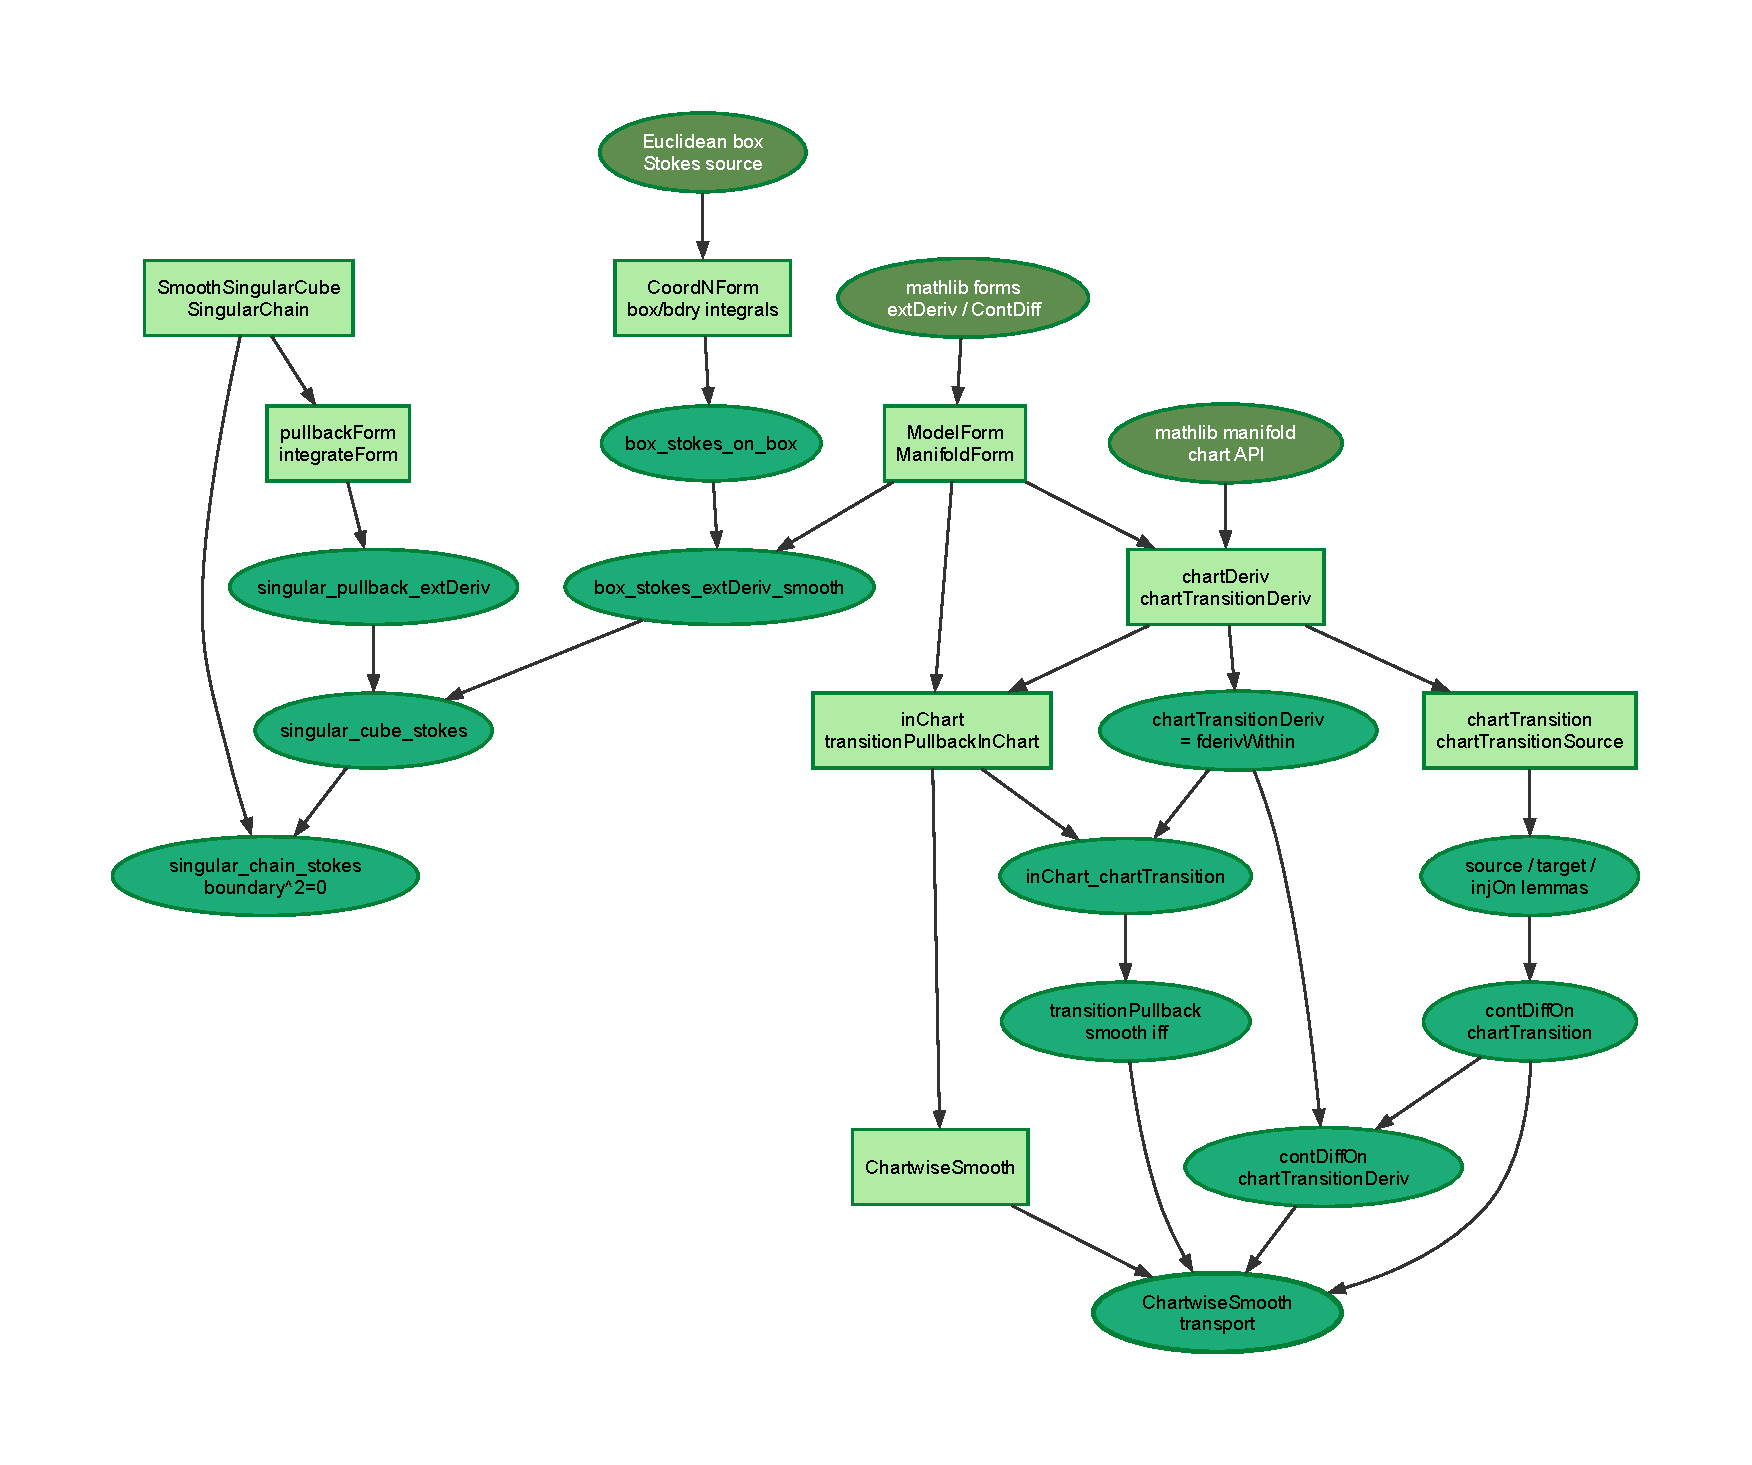
\includegraphics[width=0.92\textwidth]{figures/stokes-core-graph.pdf}
  \caption{The compactness and refinement core: compact support gives a finite
  selected cover; support-controlled partitions and smooth refinements prepare
  the local half-space Stokes data.  Light-green rectangular nodes denote
  definitions or constructed data; dark-green oval nodes denote theorem-level
  statements or derived equalities.}
  \label{fig:core-graph}
\end{figure}

\subsection{Why finite data is not bookkeeping}

The finite selected data is the skeleton of the represented theorem.  It
determines the index types of the endpoint sums, the coefficients of the
localized forms, the boxes on which local Stokes is applied, and the support
facts used to remove artificial faces.  A mismatch between any two of these
finite structures would make the final reconstruction theorem false or
unusable.

The first-principles theorem hides the finite data from users because Lean
constructs it internally.  It does not make the data irrelevant.  The data is
the mechanism by which compact support becomes a finite coordinate Stokes
proof.

In this sense, compactness is not a side condition of Stokes but a generator
of the proof route.  It selects the charts, fixes the partition coefficients,
determines which boundary carriers are active, and supplies the index sets for
the represented endpoints.  The final theorem can have a small input because
this generated finite data is coherent by construction.

\begin{remark}
The support-controlled partition is the reason compactness can be used once,
near the beginning of the proof, rather than reintroduced as local hypotheses
for every box.  Once the finite selected data is built, all later support facts
are consequences of the selected construction.
\end{remark}
